% Options for packages loaded elsewhere
\PassOptionsToPackage{unicode}{hyperref}
\PassOptionsToPackage{hyphens}{url}
%
\documentclass[
]{book}
\usepackage{amsmath,amssymb}
\usepackage{lmodern}
\usepackage{iftex}
\ifPDFTeX
  \usepackage[T1]{fontenc}
  \usepackage[utf8]{inputenc}
  \usepackage{textcomp} % provide euro and other symbols
\else % if luatex or xetex
  \usepackage{unicode-math}
  \defaultfontfeatures{Scale=MatchLowercase}
  \defaultfontfeatures[\rmfamily]{Ligatures=TeX,Scale=1}
\fi
% Use upquote if available, for straight quotes in verbatim environments
\IfFileExists{upquote.sty}{\usepackage{upquote}}{}
\IfFileExists{microtype.sty}{% use microtype if available
  \usepackage[]{microtype}
  \UseMicrotypeSet[protrusion]{basicmath} % disable protrusion for tt fonts
}{}
\makeatletter
\@ifundefined{KOMAClassName}{% if non-KOMA class
  \IfFileExists{parskip.sty}{%
    \usepackage{parskip}
  }{% else
    \setlength{\parindent}{0pt}
    \setlength{\parskip}{6pt plus 2pt minus 1pt}}
}{% if KOMA class
  \KOMAoptions{parskip=half}}
\makeatother
\usepackage{xcolor}
\IfFileExists{xurl.sty}{\usepackage{xurl}}{} % add URL line breaks if available
\IfFileExists{bookmark.sty}{\usepackage{bookmark}}{\usepackage{hyperref}}
\hypersetup{
  pdftitle={Presentations by Colin Madland},
  pdfauthor={Colin Madland},
  hidelinks,
  pdfcreator={LaTeX via pandoc}}
\urlstyle{same} % disable monospaced font for URLs
\usepackage{longtable,booktabs,array}
\usepackage{calc} % for calculating minipage widths
% Correct order of tables after \paragraph or \subparagraph
\usepackage{etoolbox}
\makeatletter
\patchcmd\longtable{\par}{\if@noskipsec\mbox{}\fi\par}{}{}
\makeatother
% Allow footnotes in longtable head/foot
\IfFileExists{footnotehyper.sty}{\usepackage{footnotehyper}}{\usepackage{footnote}}
\makesavenoteenv{longtable}
\usepackage{graphicx}
\makeatletter
\def\maxwidth{\ifdim\Gin@nat@width>\linewidth\linewidth\else\Gin@nat@width\fi}
\def\maxheight{\ifdim\Gin@nat@height>\textheight\textheight\else\Gin@nat@height\fi}
\makeatother
% Scale images if necessary, so that they will not overflow the page
% margins by default, and it is still possible to overwrite the defaults
% using explicit options in \includegraphics[width, height, ...]{}
\setkeys{Gin}{width=\maxwidth,height=\maxheight,keepaspectratio}
% Set default figure placement to htbp
\makeatletter
\def\fps@figure{htbp}
\makeatother
\setlength{\emergencystretch}{3em} % prevent overfull lines
\providecommand{\tightlist}{%
  \setlength{\itemsep}{0pt}\setlength{\parskip}{0pt}}
\setcounter{secnumdepth}{5}
\usepackage{booktabs}
\usepackage{amsthm}
\makeatletter
\def\thm@space@setup{%
  \thm@preskip=8pt plus 2pt minus 4pt
  \thm@postskip=\thm@preskip
}
\makeatother
\ifLuaTeX
  \usepackage{selnolig}  % disable illegal ligatures
\fi
\usepackage[]{natbib}
\bibliographystyle{apalike}

\title{Presentations by Colin Madland}
\author{Colin Madland}
\date{Last updated: 2022-05-16}

\begin{document}
\maketitle

{
\setcounter{tocdepth}{1}
\tableofcontents
}
\hypertarget{welcome}{%
\chapter*{Welcome}\label{welcome}}
\addcontentsline{toc}{chapter}{Welcome}

Please use the table of contents on the left to navigate through my presentations.

\hypertarget{otessa22---assessment-and-digital-technology-in-higher-education}{%
\chapter*{OTESSA22 - Assessment and Digital Technology in Higher Education}\label{otessa22---assessment-and-digital-technology-in-higher-education}}
\addcontentsline{toc}{chapter}{OTESSA22 - Assessment and Digital Technology in Higher Education}

\hypertarget{introduction}{%
\section*{Introduction}\label{introduction}}
\addcontentsline{toc}{section}{Introduction}

\hypertarget{colin-madland-phd-candidate-university-of-victoria}{%
\subsection*{Colin Madland, PhD Candidate, University of Victoria}\label{colin-madland-phd-candidate-university-of-victoria}}
\addcontentsline{toc}{subsection}{Colin Madland, PhD Candidate, University of Victoria}

\textbf{Presented Online at OTESSA22, May 17, 2022}

\begin{quote}
I acknowledge that the land where I currently live and work remains the traditional, ancestral, and unceded land of the \texttt{syilx} people, whose historical stewardship of and connections to the land continue to today. I am grateful to be an uninvited guest on this land.
\end{quote}

\begin{figure}
\centering
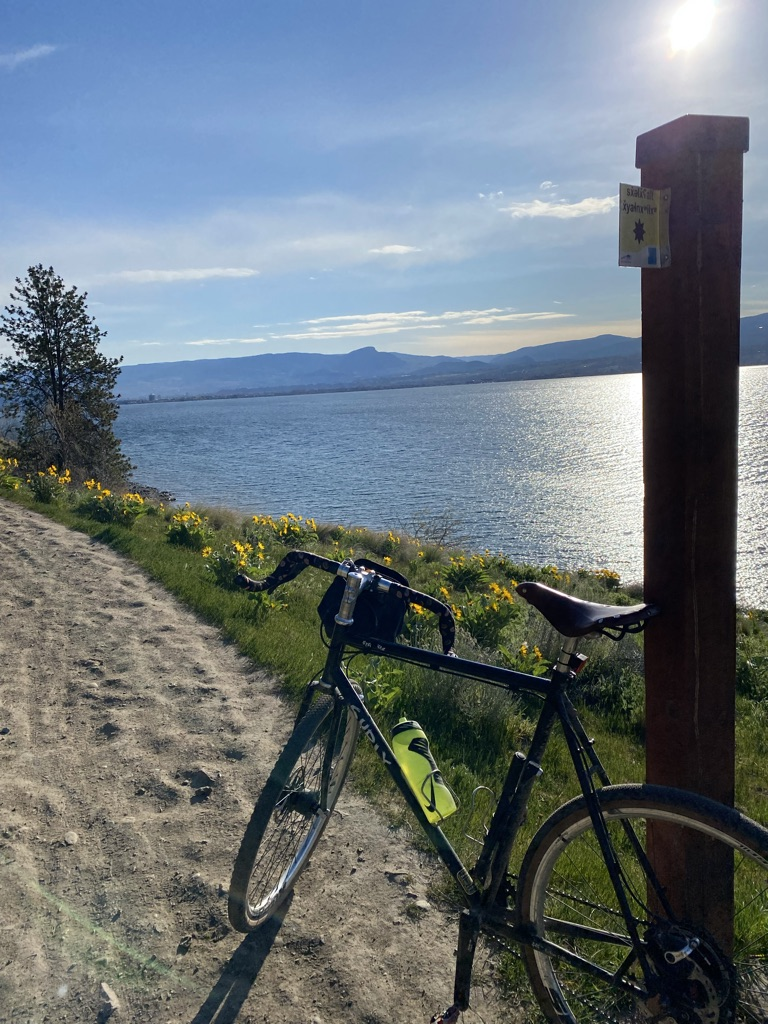
\includegraphics{assets/otessa22/kalamoir.jpg}
\caption{Picture of a bicycle resting against a pole along a trail in Kalamoir Park overlooking Okanagan Lake.}
\end{figure}

\hypertarget{background}{%
\subsection*{Background}\label{background}}
\addcontentsline{toc}{subsection}{Background}

\hypertarget{scriven-1967}{%
\subsubsection*{Scriven, 1967}\label{scriven-1967}}
\addcontentsline{toc}{subsubsection}{Scriven, 1967}

\begin{quote}
Scriven, M. (1967). \emph{The methodology of evaluation.} In B. O. Smith (Ed.), \emph{Perspectives of curriculum evaluation}. Rand McNally
\end{quote}

\begin{itemize}
\tightlist
\item
  distinction between \texttt{formative} and \texttt{summative}
\end{itemize}

\hypertarget{bloom-1968}{%
\subsubsection*{Bloom, 1968}\label{bloom-1968}}
\addcontentsline{toc}{subsubsection}{Bloom, 1968}

\begin{quote}
Bloom, B. (1968). Learning for Mastery. Instruction and Curriculum. Regional Education Laboratory for the Carolinas and Virginia, Topical Papers and Reprints, Number 1. \emph{Evaluation Comment, 1}(2), 12.
\end{quote}

\begin{itemize}
\tightlist
\item
  Incorporated \texttt{formative} and \texttt{summative} distinction into his ideas about \texttt{mastery\ learning}
\end{itemize}

\hypertarget{mislevy-1994}{%
\subsubsection*{Mislevy, 1994}\label{mislevy-1994}}
\addcontentsline{toc}{subsubsection}{Mislevy, 1994}

\begin{quote}
Mislevy, R. J. (1994). Test theory reconcieved. \emph{ETS Research Report Series, 1994}(1), i--38. \url{https://doi.org/10/gjm236}
\end{quote}

\begin{itemize}
\item
  \begin{quote}
  test theory is machinery for reasoning from students' behavior to conjectures about their competence, as framed in a particular conception of competence.''(p.~4).
  \end{quote}
\item ~
  \hypertarget{black-and-wiliam-1998}{%
  \subsubsection*{Black and Wiliam, 1998}\label{black-and-wiliam-1998}}
  \addcontentsline{toc}{subsubsection}{Black and Wiliam, 1998}
\end{itemize}

\begin{quote}
Black, P., \& Wiliam, D. (1998). Assessment and Classroom Learning. \emph{Assessment in Education: Principles, Policy \& Practice, 5}(1), 7--74. \url{https://doi.org/10/fpnss4}
\end{quote}

\begin{itemize}
\item
  major review of the literature on \texttt{formative\ assessment}\\
\item
  describe formative assessment as encouraging gains in achievement that were

\begin{verbatim}
> among the largest ever reported for educational interventions (p. 61)
\end{verbatim}
\end{itemize}

\hypertarget{pellegrino-et-al.-2001}{%
\subsubsection*{Pellegrino et al., 2001}\label{pellegrino-et-al.-2001}}
\addcontentsline{toc}{subsubsection}{Pellegrino et al., 2001}

\begin{quote}
Pellegrino, J. W., Chudowsky, N., \& Glaser, R. (2001). \emph{Knowing What Students Know: The Science and Design of Educational Assessment}. National Academies Press. \url{https://doi.org/10.17226/10019}
\end{quote}

\begin{itemize}
\tightlist
\item
  ``a process of drawing reasonable inferences about what students know on the basis of evidence derived from observations of what they say, do, or make in selected situations'' (p.~112)\\
\item
  ``reasoning from evidence'' (p.~43)
\end{itemize}

\hypertarget{assessment-triangle}{%
\paragraph*{Assessment Triangle}\label{assessment-triangle}}
\addcontentsline{toc}{paragraph}{Assessment Triangle}

\begin{figure}
\centering
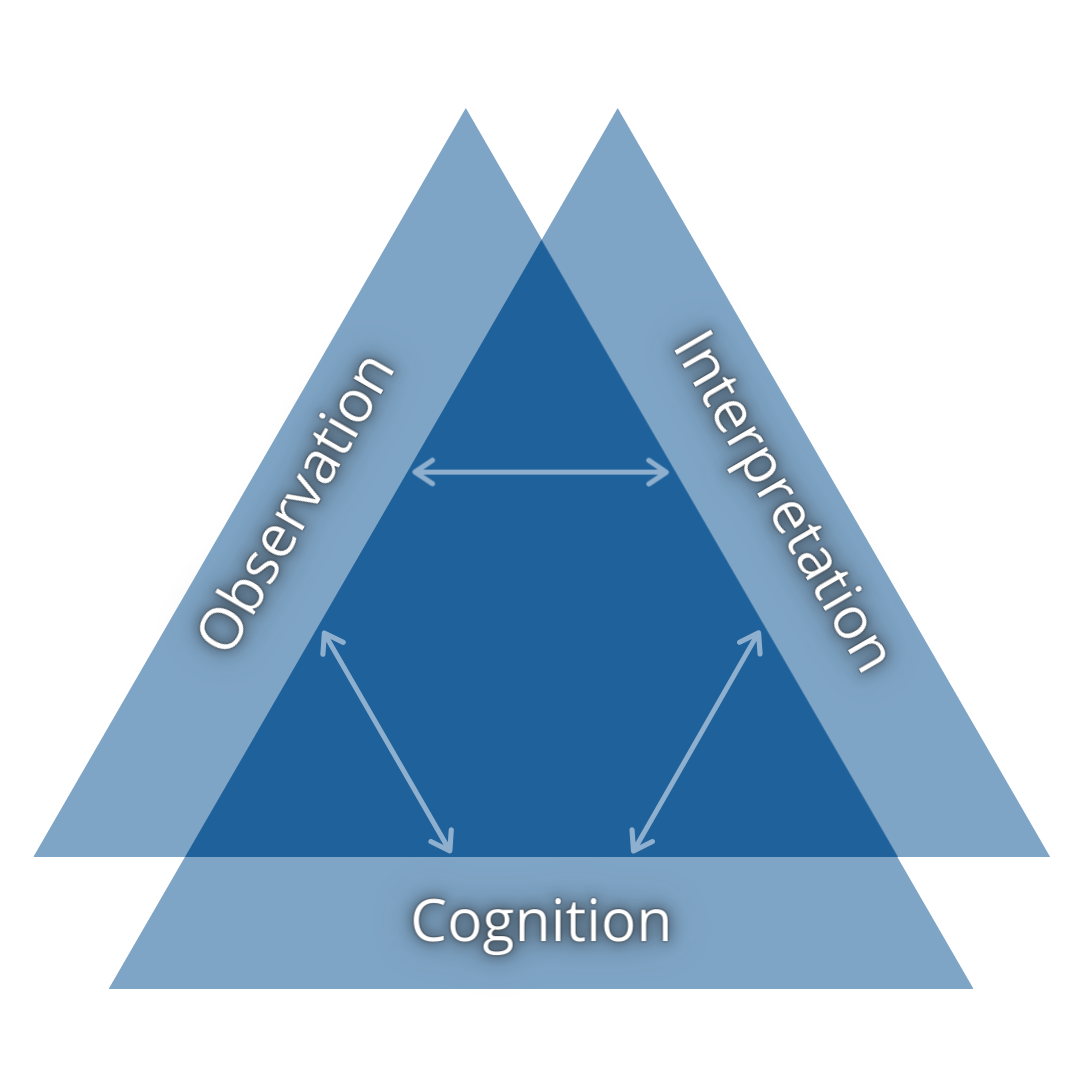
\includegraphics{assets/otessa22/assessment-triangle.png}
\caption{Stylized diagram of a triangle with the sides labeled, (clockwise from the bottom) Cognition, Observation, and Interpretation. There are two-way arrows pointing between each of the sides.}
\end{figure}

\hypertarget{cognition}{%
\subparagraph*{Cognition}\label{cognition}}
\addcontentsline{toc}{subparagraph}{Cognition}

\begin{itemize}
\tightlist
\item
  a cognitive model of the domain
\end{itemize}

\hypertarget{observation}{%
\subparagraph*{Observation}\label{observation}}
\addcontentsline{toc}{subparagraph}{Observation}

\begin{itemize}
\tightlist
\item
  a performance task used to gather data regarding learner achievement
\end{itemize}

\hypertarget{interpretation}{%
\subparagraph*{Interpretation}\label{interpretation}}
\addcontentsline{toc}{subparagraph}{Interpretation}

\begin{itemize}
\tightlist
\item
  an inference or judgement of the learner's achievement in relation to the model of the domain
\end{itemize}

\hypertarget{approaches-to-learning}{%
\subsection*{Approaches to Learning}\label{approaches-to-learning}}
\addcontentsline{toc}{subsection}{Approaches to Learning}

\hypertarget{biggs-1993}{%
\subsubsection*{Biggs, 1993}\label{biggs-1993}}
\addcontentsline{toc}{subsubsection}{Biggs, 1993}

\hypertarget{conceptions-of-assessment}{%
\subsection*{Conceptions of Assessment}\label{conceptions-of-assessment}}
\addcontentsline{toc}{subsection}{Conceptions of Assessment}

\hypertarget{brown-1994-1996}{%
\subsubsection*{Brown, 1994; 1996}\label{brown-1994-1996}}
\addcontentsline{toc}{subsubsection}{Brown, 1994; 1996}

\hypertarget{fletcher-et-al.-2012}{%
\subsubsection*{Fletcher et al., 2012}\label{fletcher-et-al.-2012}}
\addcontentsline{toc}{subsubsection}{Fletcher et al., 2012}

\hypertarget{assessment-in-higher-education}{%
\section*{Assessment in Higher Education}\label{assessment-in-higher-education}}
\addcontentsline{toc}{section}{Assessment in Higher Education}

\hypertarget{technology-mediated-assessment}{%
\section*{Technology-Mediated Assessment}\label{technology-mediated-assessment}}
\addcontentsline{toc}{section}{Technology-Mediated Assessment}

\hypertarget{research-directions}{%
\section*{Research Directions}\label{research-directions}}
\addcontentsline{toc}{section}{Research Directions}

  \bibliography{book.bib}

\end{document}
